% 2.3.CmakeLibrary.tex
%	Last update: 2019/07/11 F.Kanehori
%newpage
\subsection{cmakeの実行}
\label{subsec:CmakeLibrary}

\noindent
以下では、\cmake の生成物を格納する作業場所(ディレクトリ)を\build として
話を進めます(作業場所は任意で構いません)。

\medskip
\cmake にはConfigureとGenerateの2段階があります。

\medskip
\begin{narrow}[15pt]
	\CmndBox{%
		> chdir C:/Springhead\\
		> mkdir build\\
		> cmake -B build \it{generator}
	}
	コマンドプロンプトからならば、1回のコマンドで両方を実行できます。

	\bigskip
	GUIの場合は、図\ref{fig:CmakeConfigure}のConfigureボタンを押します(左図の下)。

	\begin{figure}[h]
	\begin{center}
	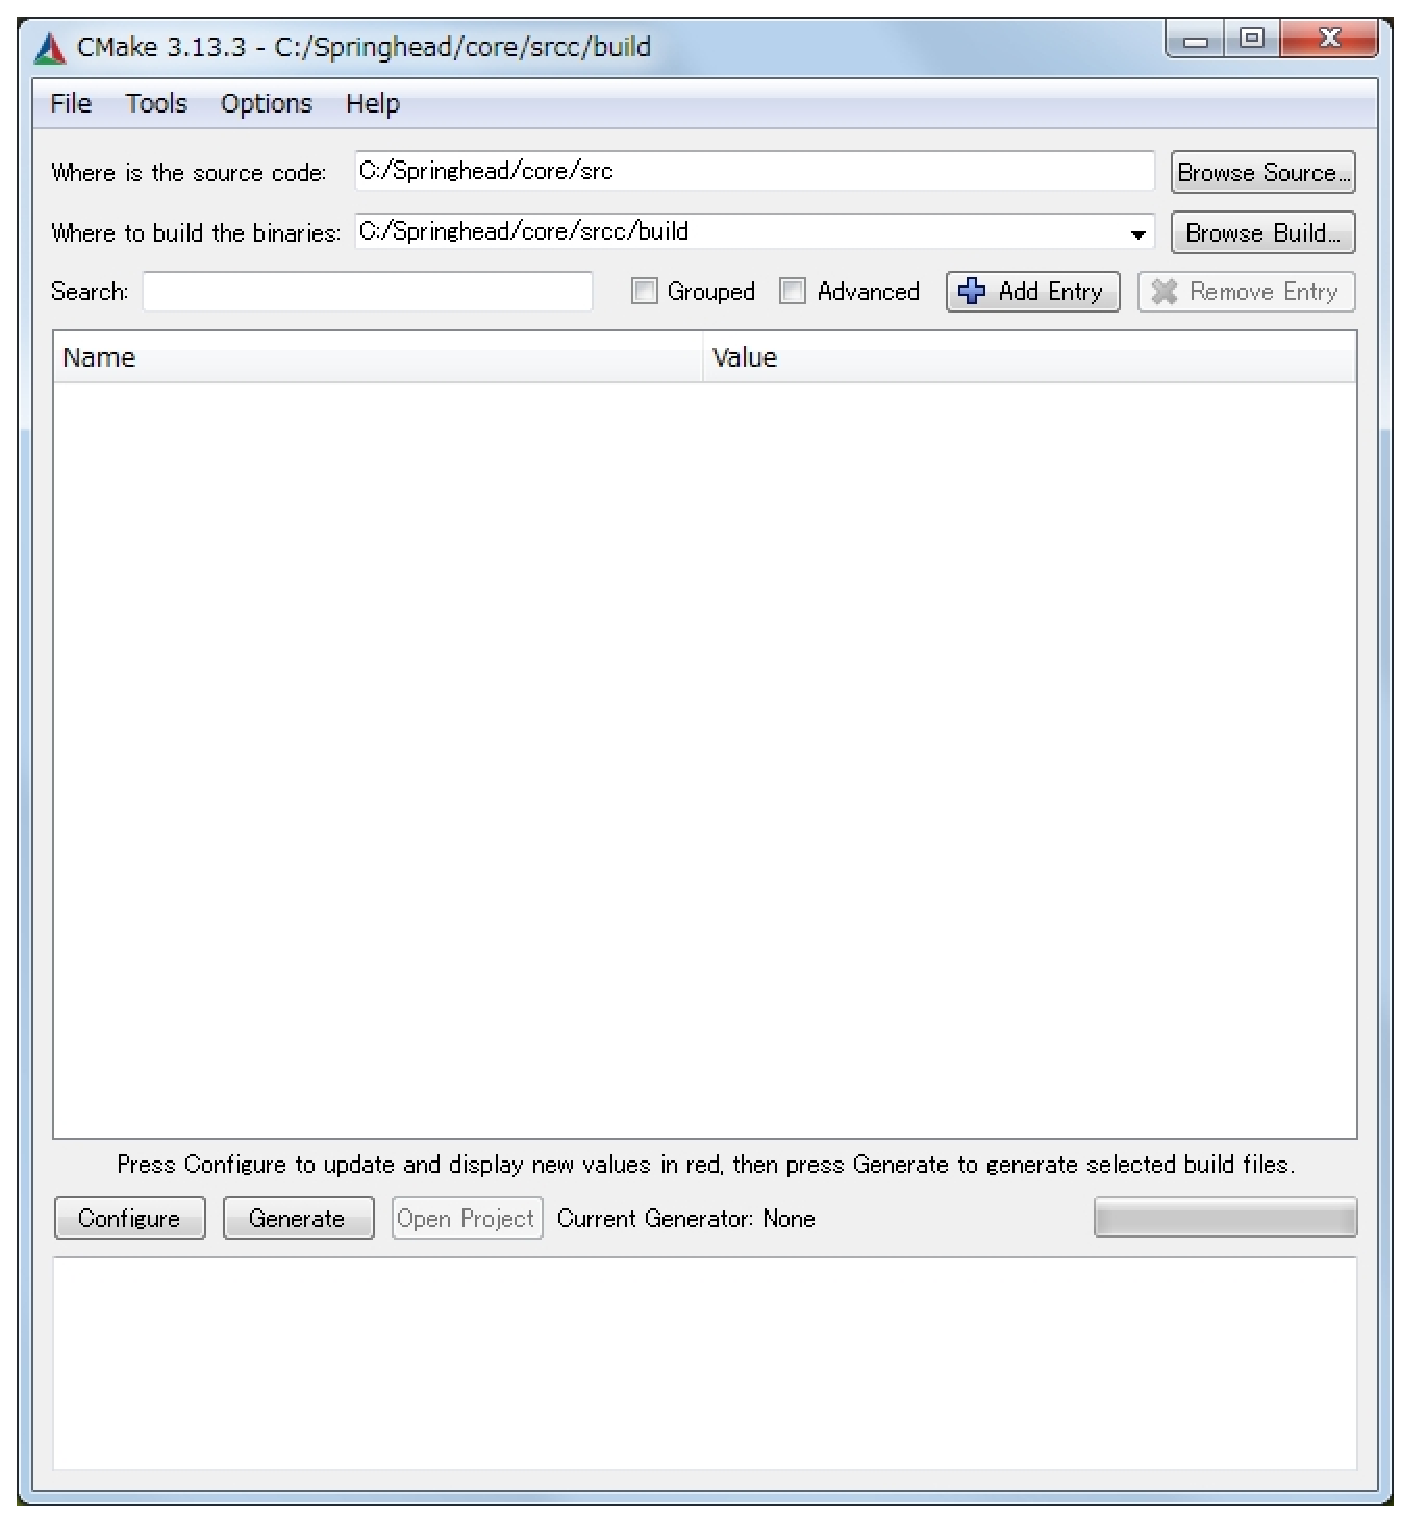
\includegraphics[width=0.35\textwidth]{fig/CmakeConfigure1.eps}
	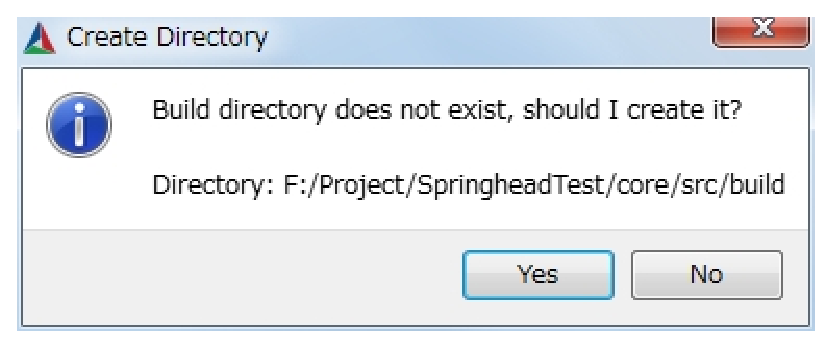
\includegraphics[width=0.2\textwidth]{fig/CmakeConfigure2.eps}
	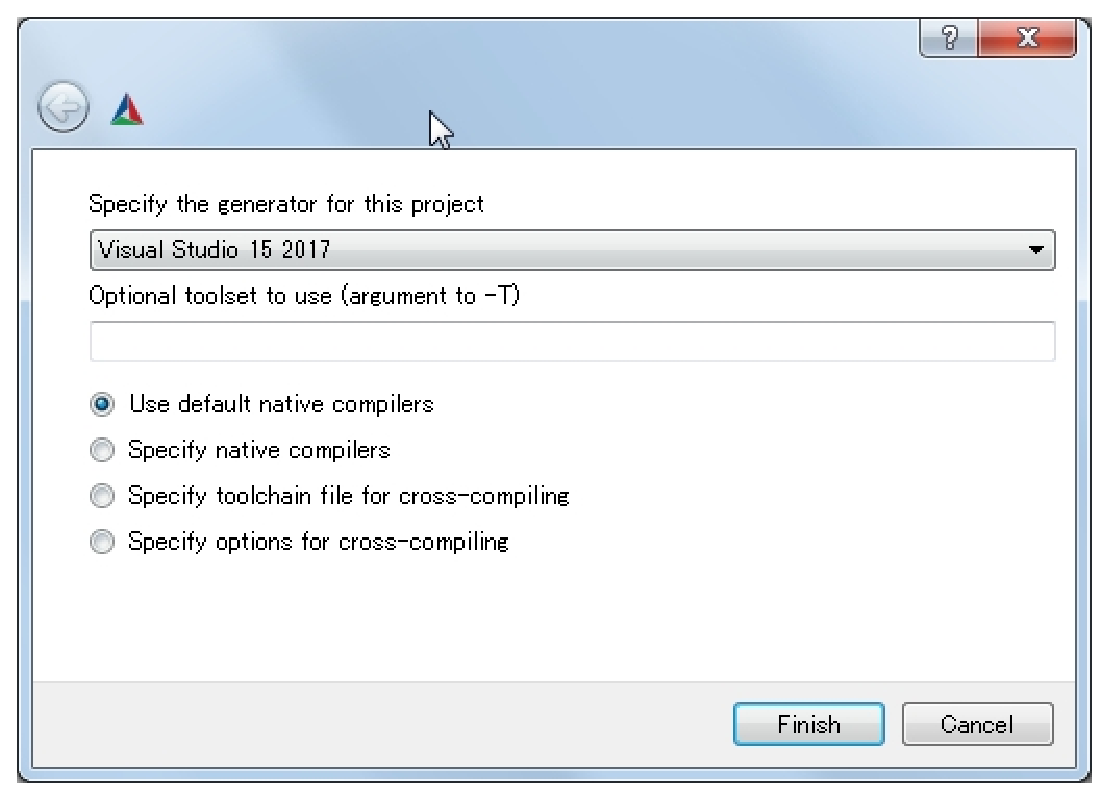
\includegraphics[width=0.3\textwidth]{fig/CmakeConfigure3.eps}
	\end{center}
	\caption{\cmake\ configure}
	\label{fig:CmakeConfigure}
	\end{figure}

	\build がなければ作成するかどうか聞かれ(中図)、
	次にgenerator指定画面となります(右図)。

	\medskip
	cmake version 3.15.0では、
	generatorとして図\ref{fig:CmakeGenerator}のものが指定できます。

	\begin{figure}[h]
	\begin{center}
	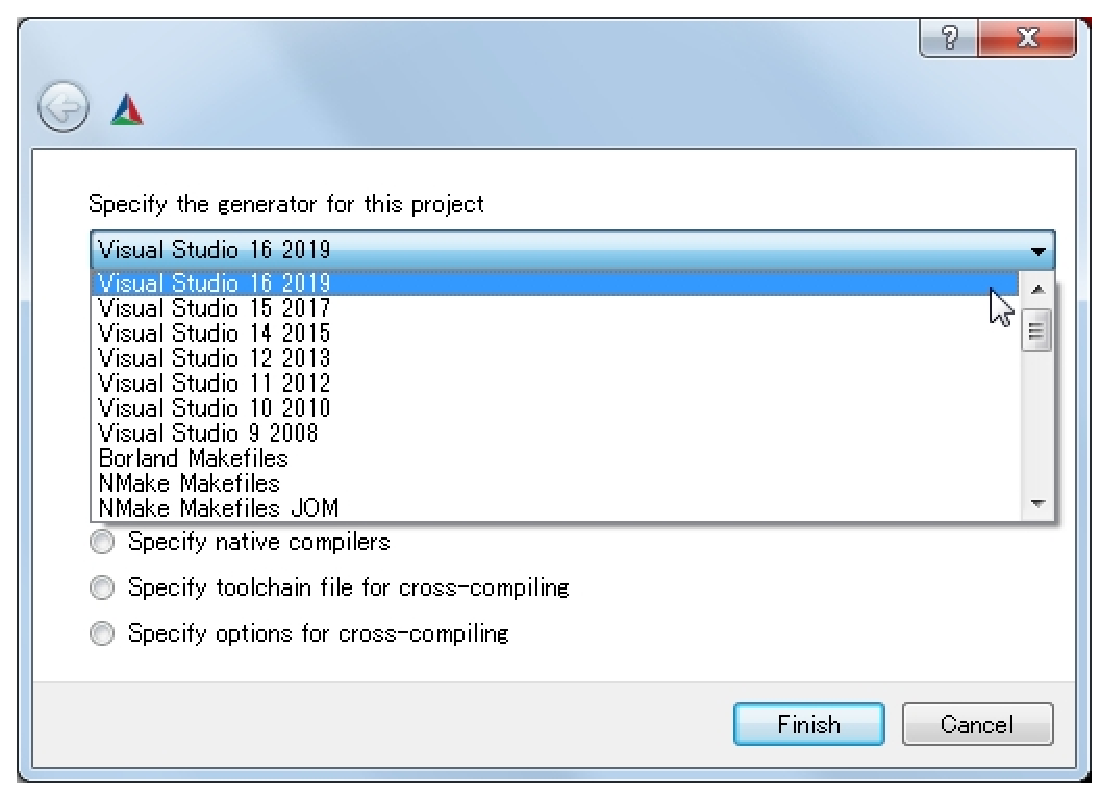
\includegraphics[width=0.3\textwidth]{fig/CmakeConfigure4.eps}
	\end{center}
	\caption{\cmake\ generator}
	\label{fig:CmakeGenerator}
	\end{figure}
	generatorの詳細については、コマンドプロンプトで
	\tt{cmake --help}として確認してください。

	次に図\ref{fig:CmakeConfigure}左図下のGenerateボタンを押します。
\end{narrow}

以上で、\build 以下にsolution/project fileなどが生成されたはずです。

% end: 2.3.CmakeLibrary.tex
